\documentclass[12pt]{article}
\usepackage[utf8]{inputenc}

% Importing settings from setup.sty
\usepackage{setup}
\usepackage{booktabs}
\usepackage{multicol}
\usepackage{multirow}
\usepackage{glossaries}
% \makenoidxglossaries
% \newcommand{\prox}{\operatorname{prox}}


% \pagenumbering{roman}
\begin{document}

% Inserting title page
\import{./}{title}

\pagenumbering{gobble}
\tableofcontents
% \listoffigures
% \listoftables



\newgeometry{
  left=25mm,
  right=25mm,
  top=25mm,
  bottom=25mm}
\pagenumbering{arabic}
 
% Evaluation: Write a brief report in which you provide your own view of the challenge of "Learning Without Data Collections". The report can be based on my book entitled "DEEP LEARNING TO SEE - Towards New Foundations of Computer Vision" and on both my two lectures. In particular you could organized you report as follows:

% 1. Brief discussion on actual contexts in which  the view of  "Learning Without Data Collections" can take place.
% 2. Critical comments on the notion of motion invariance. In particular, provide a perspective on strengths and weakness in the process of feature extraction
% 3. Find one-two articles that you consider related to the covered topic and underline the similarities.

% Frogs' eyes can't see what doesn't move.
% AI are really good (performance), but really bad (computational cost)

\section{Introduction}
``Learning without data collection'' is a provocative way to describe the process of learning from a single, or very few example. Humans however, are able to learn in such a way. Algorithms on the other hand, especially deep learning ones, are very data-hungry even for simple tasks such as recognising a cat from a dog.

\section{Context of Learning without Data Collection}
\label{sec: in favor of MI}
In this section, we will give some context to the notion of learning without data collection and we will introduce the notion of motion invariance. We will see that motion invariance turns out to be quite useful in terms of efficiency, especially when Human performance is compared to deep learning algorithms.

\subsection{A bit of context}
Learning without data collection can be applied to many fields within machine learning. One notable example is the field of computer vision. When humans see a object moving, they are almost imidiately able to recognise it. We do not require hundreds of thousands of examples in order to identify it. One iteresting thing however is that, when we see a paused video, on a phone or a computer screen for instance, we are sometimes incapable of recognising objects. Think of a paused video about a jaguar in the jungle. The jaguar may be partially, or almost completely hidden. In this case, it may be difficult to identify it. When we turn the video on, it may still be challenging to see the jaguar if he is immobile. However, as soon as the jaguar starts moving, we are able to identify it. This is because of motion invariance \cite{gori2022}, which informs us of the consistency of an object (the jaguar in this case) through time.

\subsection{Motion invariance}
Indeed, we know that the paws, the ears, the tail and all other body parts of the jaguar will not start splitting up or drastically changing shape as time goes. By the principles of motion invariance, nature somehow gives us a huge amount of information at one, for free. This hints that the current state of the art in computer vision is far from the best we can achieve, as it is already far from human level with respect to data efficiency. We can note that on the one hand, deep learning already beats the best medical doctors when it comes to detecting some types of cancer \cite{shen2019}. On the other hand however, as deep learning requires large quantities of data, humans are more efficient in this regard. As such, we arrive to the somewhat contradictory conclusion that \textbf{deep learning is both better-performing (in terms of accuracy) and worse-performing (in terms of data efficiency) than humans}.

\section{Critical comments on the notion of motion invariance}
We saw in section \ref{sec: in favor of MI} that motion invariance is a gift of nature that Humans are able to use to achieve better efficiency than deep learning algorithms, although with large quantities of data such algorithms are sometimes able to outperform humans. In this section, we will see that motion invariance also has its flaws: although it may be necessary, it is not sufficient for perfect recognition in all cases.

\subsection{Motion invariance is not sufficient}
In the example of the jaguar considered previously, we see that motion invariance is not sufficient. Indeed, it requires that the object is moving. If the object is not moving, motion invariance will not be able to help us. This is because motion invariance is a property of the object as it goes through time. Let us consider a famous pathological example of the flaws of motion invariance \cite{gori2022}. Due to the biological properties of its vision, a frog is not able to see what does not move. As a result, a frog could be surrounded by food and still starve to death if the food is immobile. This example illustrates the fact that there has to be more than just motion invariance to achieve perfect recognition. One other important element is the notion of attention, in the sense that we need to focus on the right part of the image in order to recognise the object. 

\subsection{Focus of attention}
\subsubsection{Introduction to the focus of attention}
The concept of attention is illustrated by the natural phenomenon of the focus of attention. The concept of \textbf{focus of attention} refers to the ability to selectively concentrate on specific aspects of the visual scene. This is to some extent what Convolutional Neural Networks \cite{lecun1995} and transformers \cite{vaswani2017} intend to do, but the amount of data needed for these networks to perform well demonstrates that we are still very far from the Holy Grail of (at least) human-level efficiency. \\
The human capability to use the focus of attention is allowed by the cones in our eyes. These cones are responsible for the color vision. They are able to detect the presence of a specific color in a given area of the visual field (somehow like channels in a Convolutional Neural Network).

\subsubsection{The duck-rabbit illusion}
The duck-rabbit illusion is a famous ambiguous image in which both a duck and a rabbit can be seen, depending on one's point of view. An illustration of the duck-rabbit illusion is provided in figure \ref{fig: duck-rabbit}.
\begin{figure}[ht]
  \centering
  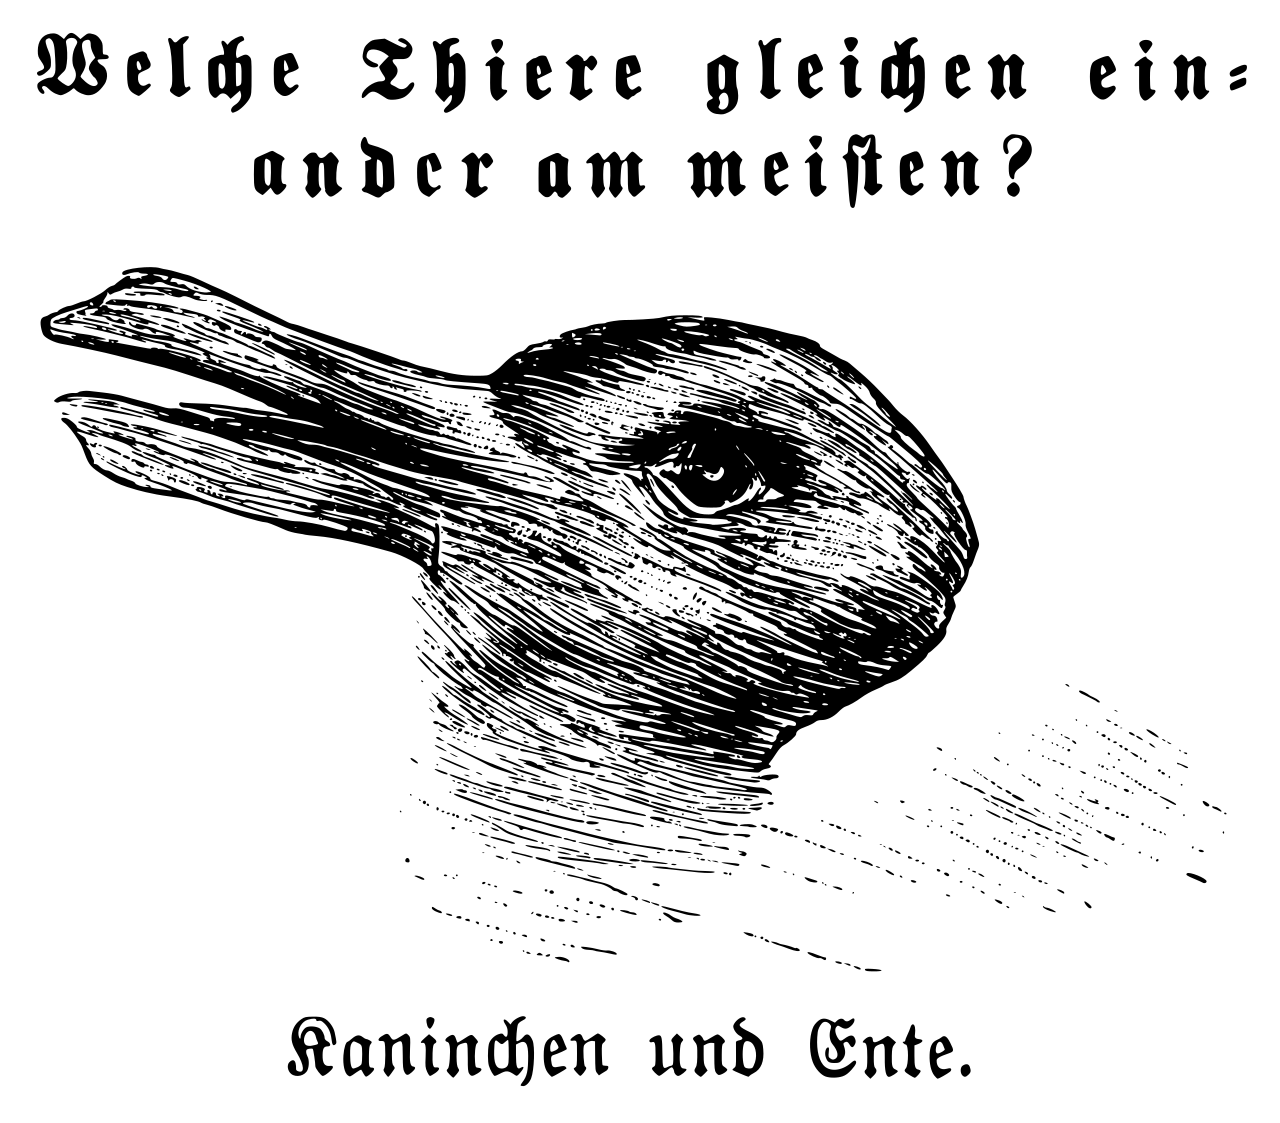
\includegraphics[width=0.5\textwidth]{images/rabbit_duck.png}
  \caption{"Kaninchen und Ente" (``Rabbit and Duck") from the 23 October 1892 issue of Fliegende Blätter}
  \label{fig: duck-rabbit}
\end{figure}
The concept was used by the Polish psychologist Joseph Jastrow, before the image was made famous by the Austrian philosopher Ludwig Wittgenstein.

\section{Conclusion}



% \clearpage
% \printnoidxglossaries
\newpage
\begin{thebibliography}{99}
  \bibitem{gori2022} Betti, A., Gori, M. and Melacci, S., 2022. Deep Learning to See: Towards New Foundations of Computer Vision. arXiv preprint arXiv:2206.15351. 
  \bibitem{shen2019} Shen, L., Margolies, L.R., Rothstein, J.H., Fluder, E., McBride, R. and Sieh, W., 2019. Deep learning to improve breast cancer detection on screening mammography. Scientific reports, 9(1), p.12495. 
  \bibitem{lecun1995} LeCun, Y. and Bengio, Y., 1995. Convolutional networks for images, speech, and time series. The handbook of brain theory and neural networks, 3361(10), p.1995.
  \bibitem{vaswani2017} Vaswani, A., Shazeer, N., Parmar, N., Uszkoreit, J., Jones, L., Gomez, A.N., Kaiser, L. and Polosukhin, I., 2017. Attention is all you need. Advances in neural information processing systems, 30.
\end{thebibliography}
\end{document}

